\documentclass{article}

\usepackage[T1]{fontenc}    %Schriftart des Dokumentes
\usepackage[ngerman]{babel} %Dokumentensprache, hier Deutsch
\usepackage{amsmath, amssymb, stmaryrd} %mathematische Schriftzeichen
\usepackage{graphicx} %Einfügen von Grafiken
\usepackage{wrapfig}
\usepackage{bm}
\usepackage{subfig}
\usepackage{newclude}
\usepackage{pdfpages}

\setlength{\parindent}{0pt} %Einrückung von Absätzen auf null gesetzt
\setlength{\parskip}{10pt} %Abstand zischen Absätzen auf 10pt gesetzt

\title{Versuch 255: Röntgenspektrometer}
\author{Matthias Kuntz}
\date{22.04.2024}

\renewcommand*\contentsname{Zusammenfassung}

\begin{document}

\maketitle

\tableofcontents

\newpage

%-------------------------EINLEITUNG-------------------------
\section{Einleitung}

Eine wichtige Eigenschaft von Kristallen in der Forschung ist ihre eindeutige und sich immer gleich wiederholende Gitter- beziehungsweise Kristallstruktur. Um diese zu untersuchen dient die Röntgenspektroskopie, bei der ein Kristall Röntgenstrahlung ausgesetzt und das reflektierte Spektrum analysiert wird. Dies ermöglicht eine qualitative Analyse des Gitterspektrums, die Bestimmung natürlicher Konstanten wie dem Planck'schen Wirkungsquantum oder der Avogadrozahl und die Vermessung verschiedener charakteristischer Linien des reflektierten Röntgenspektrums. Um all dies soll es in diesem Versuch gehen, sodass dieser als Einführung in die Themen der Röntgenstrahlung und Streuung an Kristallgittern dient.

\subsection{Physikalische Grundlagen}

\subsubsection{Röntgenröhre und Moseley'sches Gesetz}

Grundbaustein dieses Versuchs ist die Röntgenröhre. Diese besteht aus zwei Elektroden in einem evakuierten Glaskolben. Hierbei werden Elektronen durch eine Glühemission von der Anode losgelöst und über eine Beschleunigungsspannung zur Kathode bewegt, wo diese am Coulombfeld der Kathodenatome abgebremst werden und abprallen. Die dabei freiwerdende Energie zeigt sich in Form eines kontinuierlichen elektromagnetischen Bremsspektrums, welches im kurzwelligen Bereich erst oberhalb der sogenannten Grenzwellenlänge $\lambda_{gr}$ beginnt. Durchlaufenen die Elektronen die Spannung $U$ und werden dann in einem Prozess abgebremst, wodurch ihre ursprüngliche Energie $E = e U$ komplett in die Röntgenstrahlung $h \nu$ umgewandelt wird, so ergibt sich:

\begin{equation}
    E = e U = h \nu_{gr} = h  \frac{c}{\lambda_{gr}} \ \ \ \Rightarrow \ \ \ \lambda_{gr} = \frac{h c}{e U}.
    \label{eq:1_LAMBDA_GR}
\end{equation}

Somit kann man mithilfe der Grenzwellenlänge das Planck'sche Wirkungsquant $h$ bestimmen. 

Bei hohen Beschleunigungsspannungen entsteht zusätzlich zum kontinuierlichen Bremsspektrum noch ein diskretes charakteristisches Spektrum, welches sich dem ersteren überlagert. Dieses ist abhängig vom Kathodenmaterial und entsteht, wenn bei der Kathode ein Elektron aus einer niedrigeren Schale herausgeschlagen wird und ein höheres Atom um diesen Platz aufzufüllen herabfällt und freiwerdende Bindungsenergie in Form eines Röntgenquants abstrahlt. Die dabei entstehenden charakteristischen Linien lassen sich mithilfe des Moseley'schen Gesetzes bestimmen. Demnach gilt für den Übergang von der $n$-tem auf die $m$-te Schale:

\begin{equation}
    E_{n \xrightarrow{} m} = hc R_\infty (Z-A)^2 \left( \frac{1}{m^2} - \frac{1}{n^2} \right).
\end{equation}

Hierbei bezeichnen $h$ und $c$ erneut das Plank'sche Wirkungsquant sowie die Lichtgeschwindigkeit und $R_\infty$ und $Z$ bezeichnen die Rydbergenergie sowie die Kernladungszahl. $A$ steht für die Abschirmungskonstante, welche den quantenmeschanischen Effekt berücksichtigt, dass die effektive Kernladungszahl, die ein Elektron in einem Atom wahrnimmt, durch die anderen Elektronen im Atom abgeschirmt wird. Eine wichtige Anmerkung ist, dass das Moseley'sche Gesetz nur eine Abschätzung der Energie ist, da Effekte wie die Feinstrukturaufspaltung hier nicht berücksichtigt werden.  

\subsubsection{Bragg-Reflexion}

Um Röntgenstrahlung zu untersuchen verwendet man vorüberwiegend die Röntgenbeugung an Kristallen, genannt Bragg-Strahlung. Da Kristalle feste kubische Strukturen aufweisen, kann man sie als aneinandergereihte Netzebenen sehen, wobei die Strahlung an verschiednen Atomen verschiedenener Ebenen reflektiert wird, zu sehen in Abbildung \ref{fig:1_Bragg}. Das Bragg'sche Gesetz beschreibt den Zusammenhang zwischen dem Reflektionswinkel $\theta$ und der Wellenlänge der verwendeten Röntgenstrahlung $\lambda$ mithilfe des Netzebenenabstands $d$ und der Ordnungszahl $n$:

\begin{figure}[!b]
    \centering
    \resizebox{0.7\textwidth}{!}{
    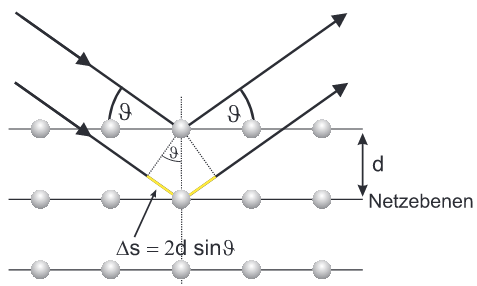
\includegraphics{graphics/bragg.png}}
    \caption{Bragg-Reflexion am Kristall [Quelle: PAP2.2 Skript, S.89, Stand:30.04.2024]}
    \label{fig:1_Bragg}
\end{figure}


\begin{equation}
    2 d \sin \theta = n \lambda, \ \ \ \ \ n \in \mathbb{N}
    \label{eq:1_BRAGG}
\end{equation}

Indem man also den Einfallswinkel und somit Ausfallswinkel der Röntgenstrahlung variiert, wird eine andere Wellenlänge der Röntgenstrahlung analysiert, wodurch es möglich wird, deren Spektrum zu messen. 

Eine weitere Anwendung der Röntgenbeugung an Kristallen dient der Bestimmung der Avogadro-Konstante $N_A$. Hierzu benötigt werden lediglich Information über Volumen und Atomanzahl einer Elementarzelle des verwendeten Kristalls. Für den von uns verwendetetn NaCl-Kristall ergibt sich die folgende Form:

\begin{equation}
    N_A = 4 \frac{V_{mol}}{V}.
\end{equation}

Hierbei bezeichnet $V_{mol}$ das Molvolumen und $V$ das Volumen einer elementarzelle. Die Zahl 4 kommt daher, dass in einer Elementarzelle eines NaCl-Kristalls vier NaCl-Moleküle vorhanden sind. $V$ kann man nun aus dem Netzebenenabstand $d$ berechnen und erhält somit unter Verwendung des Molgewichts $M_{mol}$ sowie der Dichte $\rho$:

\begin{equation}
    N_A = 4 \frac{V_{mol}}{(2d)^3} = 4 \frac{M_{mol}}{ \rho (2d)^3} = \frac{1}{2} \frac{M_{mol}}{\rho d^3}
    \label{eq:1_AVOGADRO}
\end{equation}

\newpage
\subsection{Versuchsaufbau}

Unser Versuchsaufbau besteht aus einem Röntgengerät mit Röntgenröhre, zu sehen auf der ersteen Seite im Messprotokoll. Die von der Röntgenröhre emittierte Röntgenstrahlung wird über einen Kollimator in ein Goniometer geführt, wo sie zunächst unter einem Winkel auf den befestigten Kristall und danach unter gleichem Ausfallswinkel zu einem Zählrohr geleitet wird, siehe Abbildung \ref{fig:1_Goniometer}. So können wir das Röntgenspektrum der Röntgenröhre bei verschiedenen zur Beugung verwendeten Kristallen untersuchen. Die Messungen des Zählrohrs werden digitalisiert und mithilfe der Software CASSY-LAB 2 digital analysiert und abgespeichert. 

\phantom{.}

\begin{figure}[!h]
    \centering
    \resizebox{0.8\textwidth}{!}{
    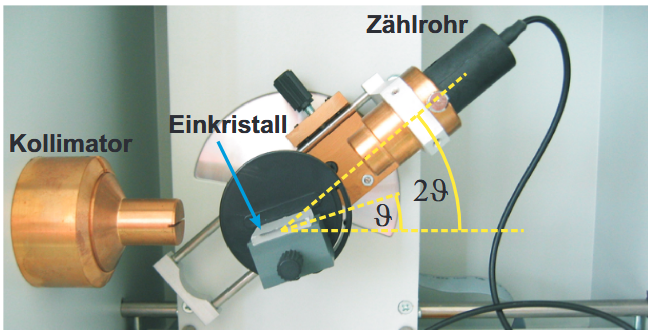
\includegraphics{graphics/goniometer.png}}
    \caption{Aufbau des Goniometers [Quelle: PAP2.2 Skript, S.91, Stand:30.04.2024]}
    \label{fig:1_Goniometer}
\end{figure}


%---------------VERSUCHSPROTOKOLL MIT MESSDATEN---------------
\newpage

\section{Versuchsprotokoll mit Messdaten}

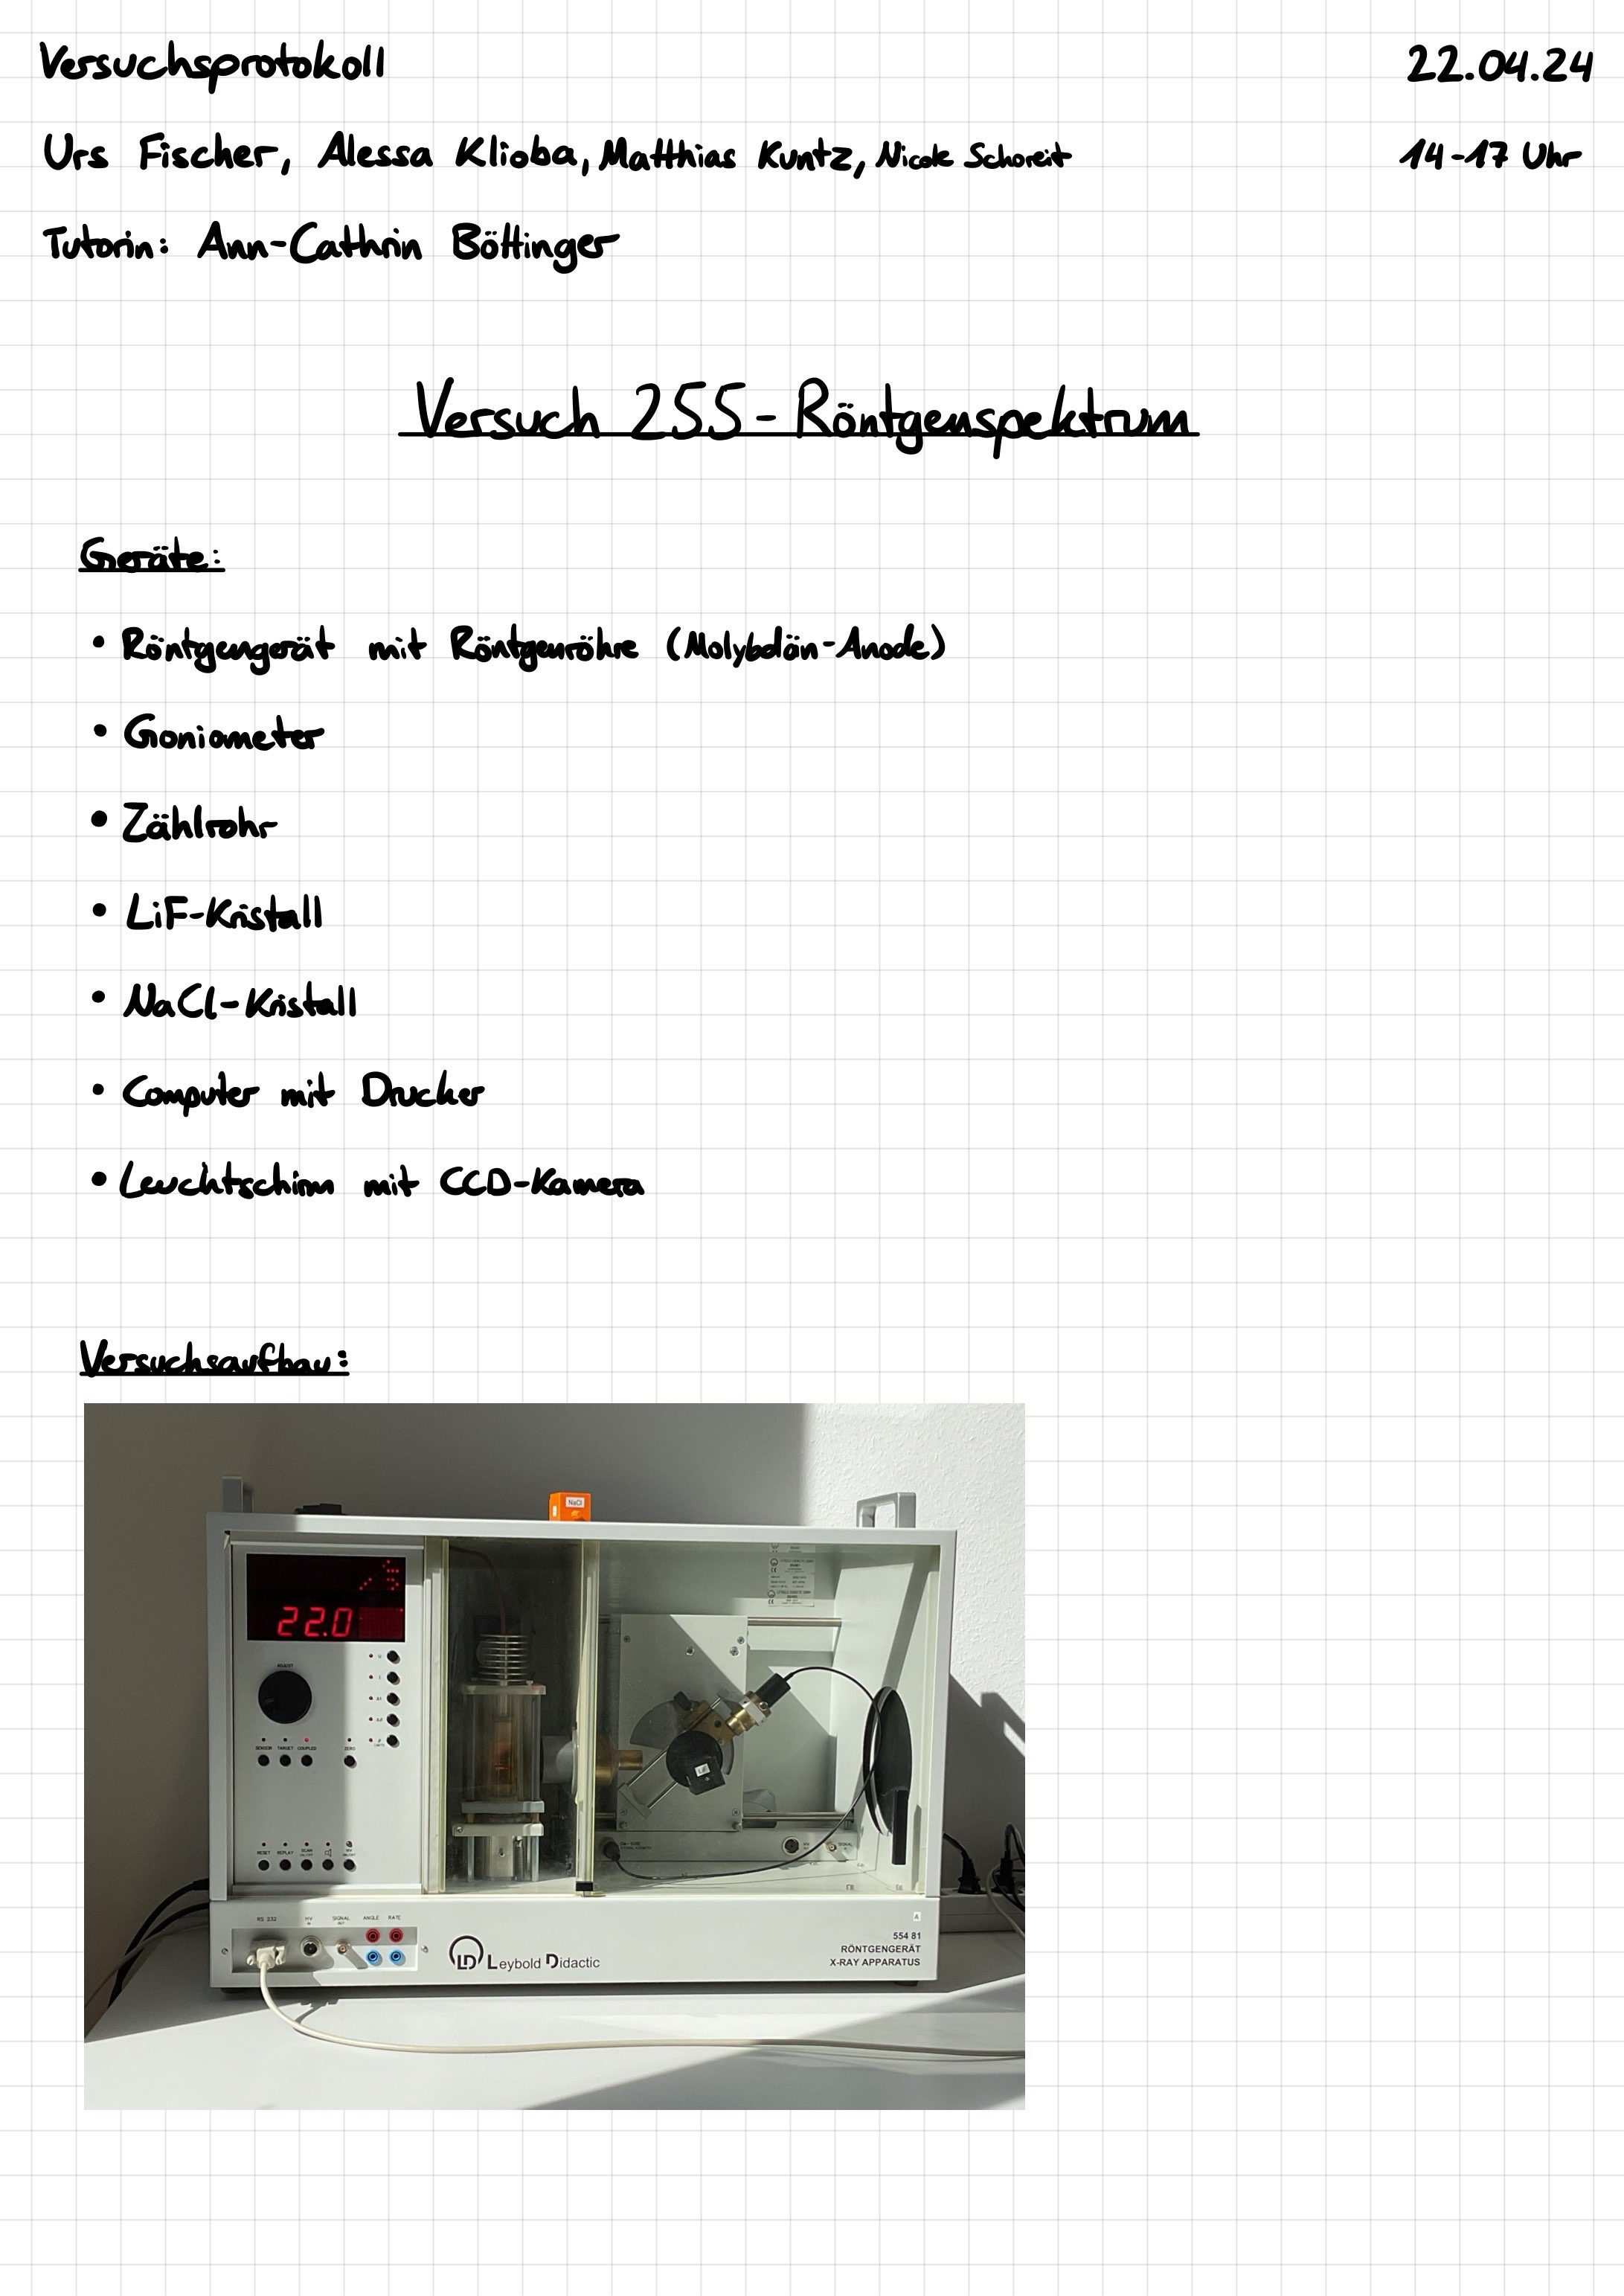
\includegraphics[width=\textwidth]{graphics/mess1.jpg}
\newpage
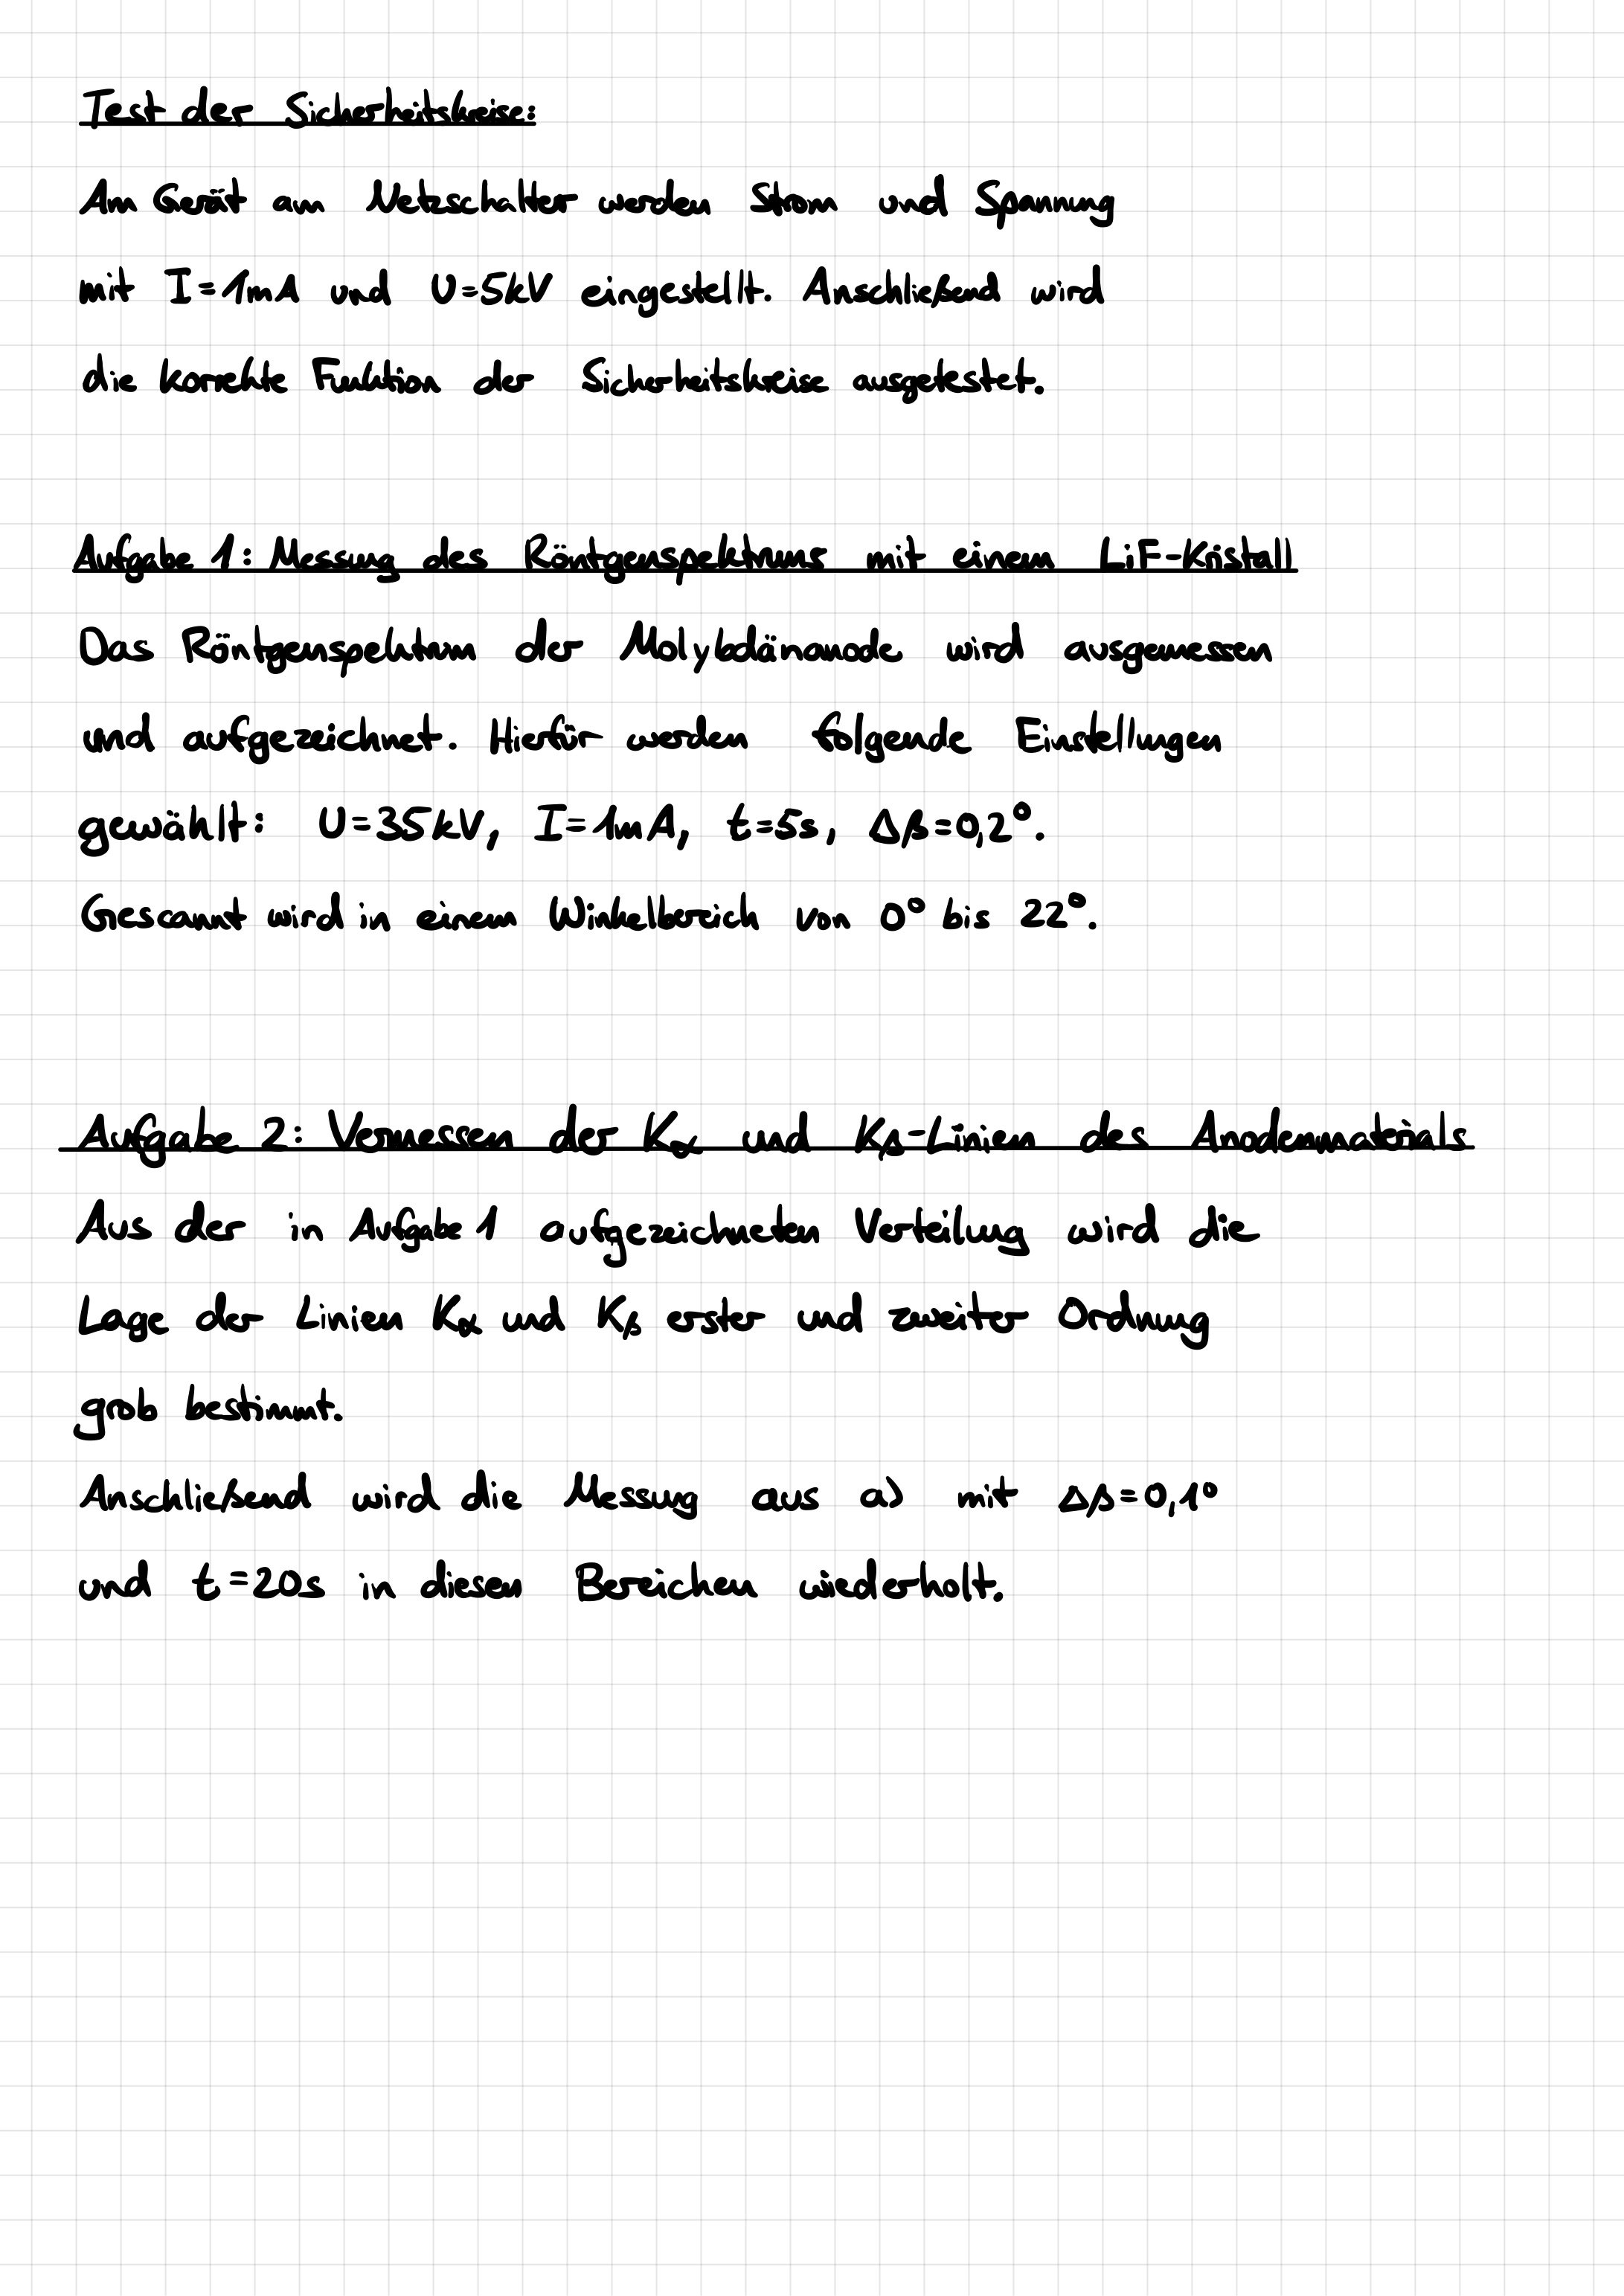
\includegraphics[width=\textwidth]{graphics/mess2.jpg}
\newpage
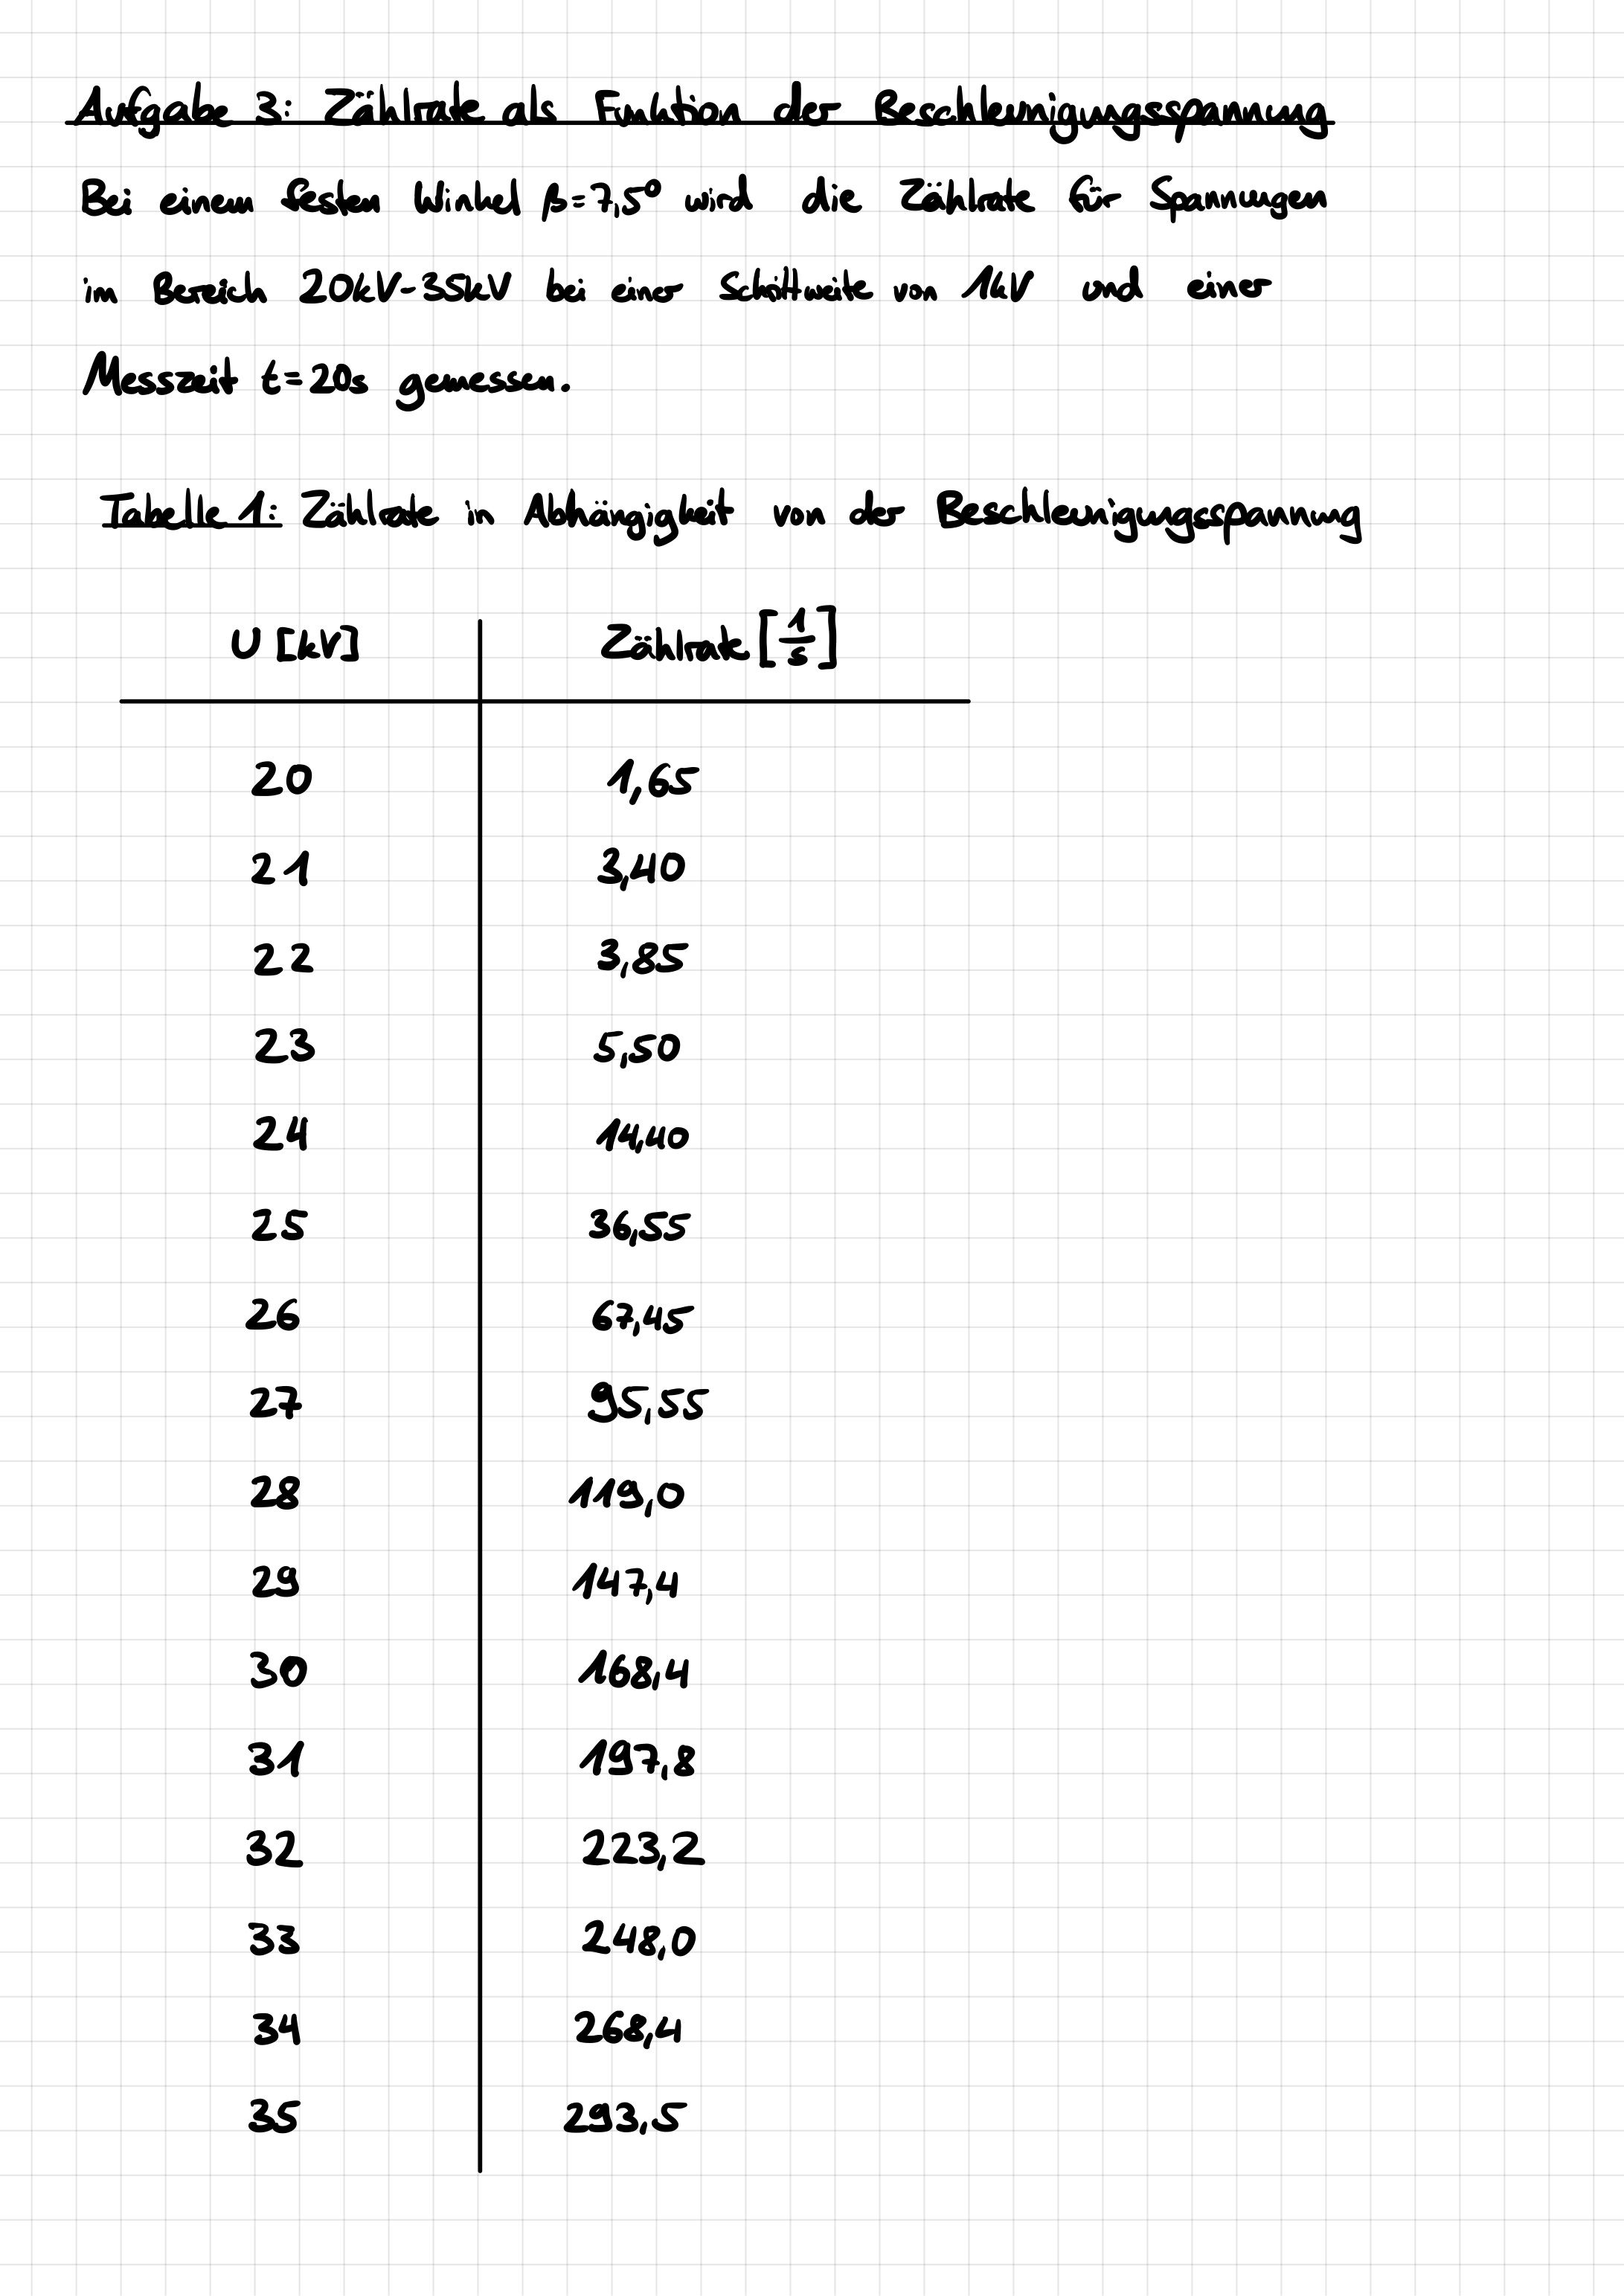
\includegraphics[width=\textwidth]{graphics/mess3.jpg}
\newpage
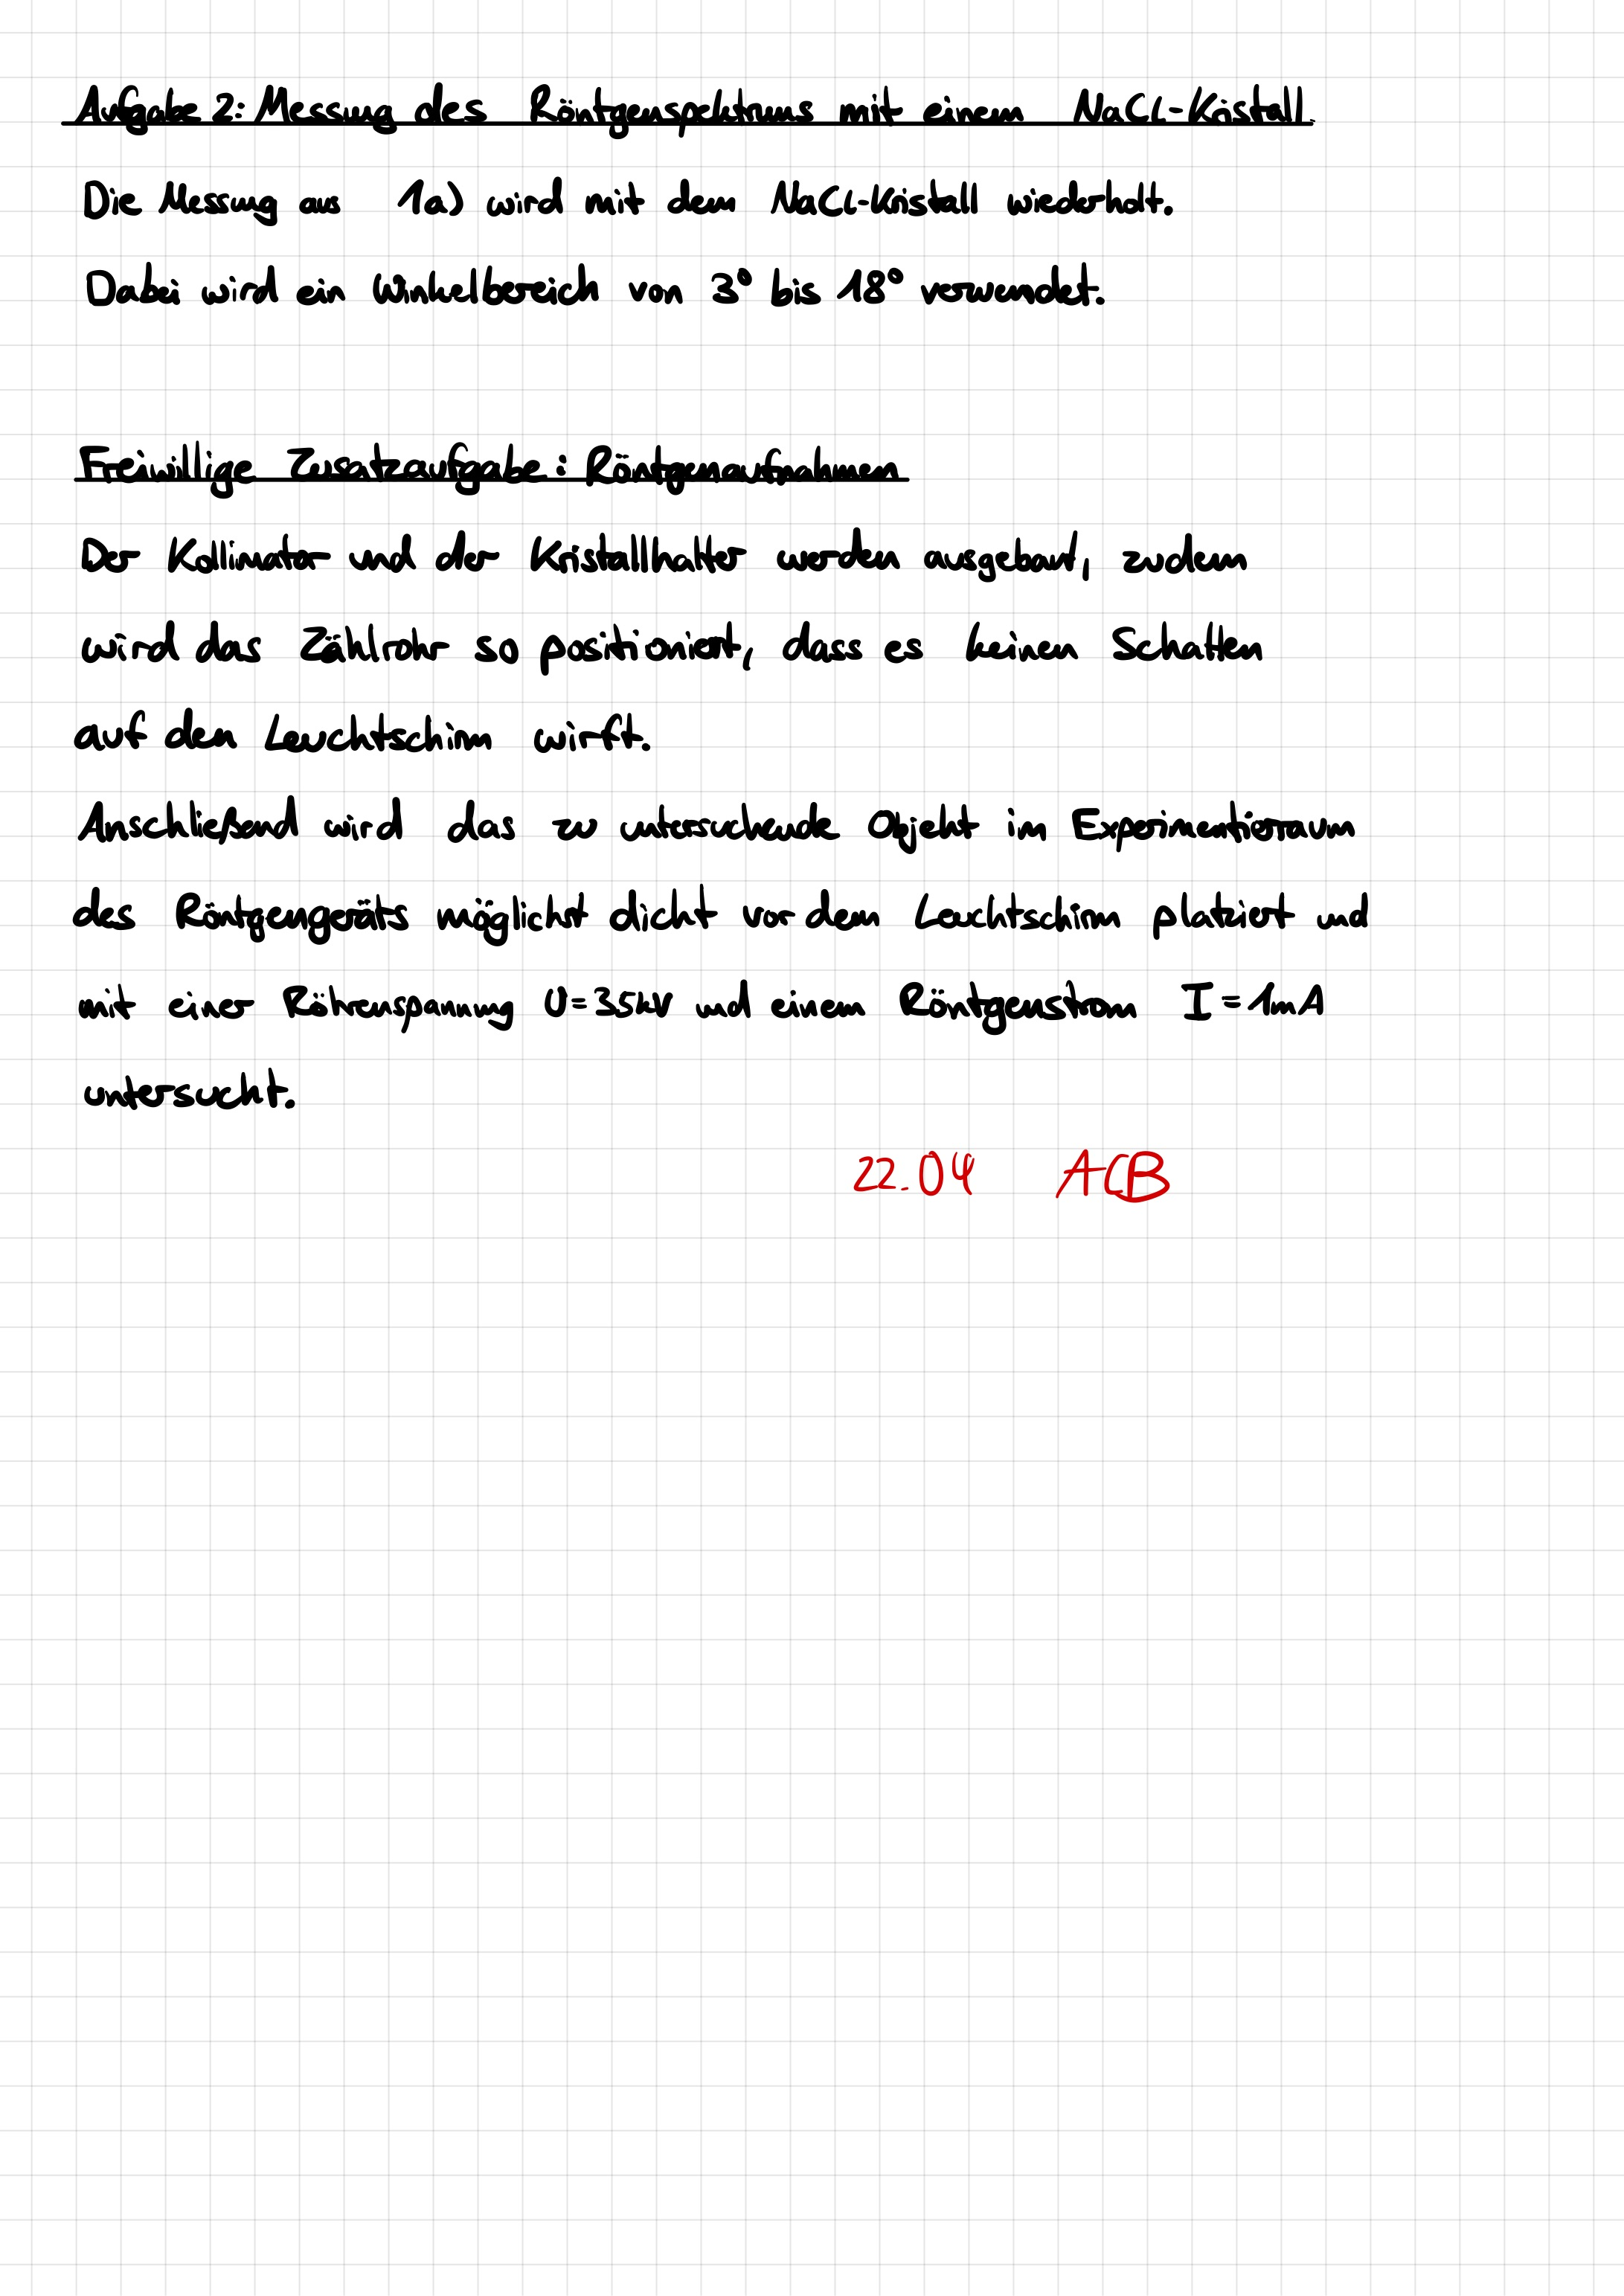
\includegraphics[width=\textwidth]{graphics/mess4.jpg}
\newpage

\addtocounter{table}{1}

\begin{figure}[p]
  \centering
  \subfloat[Campuscard]{
\includegraphics[width=0.48\textwidth]{graphics/xrays/campuscard.png}}
  \hfill
  \subfloat[Eingeschlossener Schaltkreis]{
\includegraphics[width=0.48\textwidth]{graphics/xrays/gdr.png}}
  \hfill
  \subfloat[Obere Hälfte eines Taschenrechners]{
\includegraphics[width=0.48\textwidth]{graphics/xrays/Taschenrechner oben.png}}
  \hfill
  \subfloat[Gefülltes Überraschungsei]{
\includegraphics[width=0.48\textwidth]{graphics/xrays/ü-Ei_mit_shit.png}}
  \hfill
  \caption{Verschiedene Röntgenaufnahmen}
\end{figure}

\clearpage
\newpage
%-------------------------AUSWERTUNG-------------------------
\section{Auswertung}

In dieser Evaluation werden alle Fehler, sofern keine spezifische Angabe gemacht wird, mithilfe der Gauss'schen Fehlerfortpflanzung berechnet. Dies bedeutet, dass ein Wert $F$, der mit der Formel $f(a_1, ..., a_n)$ berechnet wird, den Fehler $\Delta F$ annimmt:

\begin{equation}
    \Delta F = \sqrt{\sum_n \left( \frac{\partial f}{\partial a_n} \cdot \Delta a_n \right)^2}.
\end{equation}

Des Weiteren erfolgen Signifikanztests von zwei Werten $a$ und $a'$ über die folgende Formel:

\begin{equation}
    \sigma = \frac{|a-a'|}{\sqrt{(\Delta a)^2 + (\Delta a')^2}}.
\end{equation}

Die Auswertung sowie Berechnungen erfolgen über das dem Dokument angehängte Python-Programm.

\newpage

\subsection{Auswertung des gesamten Röntgenspektrums mit LiF-Kristall}

Wir beginnen, indem wir aus dem aufgenommenen Röntgenspektrum, zu sehen in Abbildung \ref{fig:1a} die Grenzwellenlänge $\lambda_{gr}$ bestimmen, ab der das Spektrum beginnt. Dazu normieren wir die Werte zunächst auf den Untergrund und extrapolieren darauf den annähernd linearen Verlauf im Winkelbereich von 5,0 bis 6,2°. Um den Normierungswert des Untergrunds $bkg$, welcher dann von allen Messwerten abgezogen wird, zu bestimmen fitten wir eine Konstante an die Werte bis 5,0° und erhalten so:

\begin{equation}
    bkg = (85 \pm 3) \text{counts}
\end{equation}

Wir subtrahieren also unsere Intensitätsmesswerte alle mit dem berechneten Untergrund $bkg$ und versehen diese noch mit einem Statistischen Fehler, welchen wir als 1\% des Messwerts abschätzen und mit dem Fehler des Hintergrunds quadratisch addieren:

\begin{equation}
    \Delta I = \sqrt{(0,01 \cdot I)^2 + (\Delta bkg)^2}
\end{equation}

Damit können wir nun einen linearen Fit $y = \alpha x + \beta$ an die genannten Messwerte durchführen, zu sehen in Abbildung \ref{fig:1b}. Dieser liefert die folgenden Fitparameter:

\begin{equation}
    \begin{split}
        \alpha &= (166 \pm 7) \text{counts}/{^\circ}, \\
        \beta &= -(853 \pm 38) \text{counts}. 
    \end{split}
\end{equation}

Für den Grenzwinkel $\vartheta_{gr}$ bestimmen wir die Nullstelle der Funktion:

\begin{equation}
    \begin{split}
        \vartheta_{gr} &= - \frac{\beta}{\alpha}, \\
        \Rightarrow \Delta \vartheta_{gr} &= -\vartheta_{gr} \sqrt{\left( \frac{\Delta \alpha}{\alpha} \right)^2 + \left( \frac{\Delta \beta}{\beta} \right)^2}, \\ \\
        &\Rightarrow \vartheta_{gr} = (5,1 \pm 0,3)^\circ.
    \end{split}
\end{equation}

Nun können wir mithilfe des Bragg-Gesetzes, Gleichung \ref{eq:1_BRAGG}, die Grenzwellenlänge bestimmen. Dazu verwenden wir den im Skript gegeben Wert für den Netzebenenabstand $d = 201,4 \cdot 10^{-12}$ und erhalten:

\begin{equation}
    \begin{split}
        \lambda_{gr} &= 2 d \sin{\vartheta_{gr}}, \\
        \Rightarrow \Delta \lambda_{gr} &= 2 d \cos{\vartheta_{gr}} \cdot \Delta \vartheta_{gr}, \\ \\
        &\Rightarrow \bm{\lambda_{gr} = (3,60 \pm 0,22) \cdot 10^{-11}} \textbf{m}.
    \end{split}
\end{equation}

Abschließend nutzen wir Gleichung \ref{eq:1_LAMBDA_GR} um das Planck'sche Wirkungsquant $h$ zu berechnen, wobei wir die verwendete Spannung von 35kV einsetzen:

\begin{equation}
    \begin{split}
        h &= \frac{ e U}{c} \lambda_{gr}, \\
        \Rightarrow \Delta h &= \frac{e U}{c} \cdot \Delta \lambda_{gr}, \\ \\
        &\Rightarrow \bm{h = (6,7 \pm 0,4) \cdot 10^{-34}} \textbf{Js}.  
    \end{split}
\end{equation}

Verglichen mit dem Literaturwert von $h_{lit} = 6,62607 \cdot 10^{-34}$ ergibt sich eine insignifikante Abweichung von $\sigma_h = 0,25$. 

Mithilfe des Bragg-Gesetzes können wir noch den Winkel berechnen, ab welchem das Spektrum zweiter Ordnung beginnt. Dazu verwenden wir unsere Grenzwellenlänge $\lambda_{gr}$ und setzen $n=2$:

\begin{equation}
    \begin{split}
        \vartheta_{gr,2} &= \arcsin{\frac{\lambda_{gr}}{d}}, \\
        \Rightarrow \Delta \vartheta_{gr,2} &= \frac{1}{\sqrt{d^2 - \lambda_{gr}^2}} \cdot \Delta \lambda_{gr}, \\ \\
        &\Rightarrow \bm{\vartheta_{gr,2} = (10,3 \pm 0,6)^\circ}.  
    \end{split}
\end{equation}

Dieser Wert zeigt im Vergleich mit dem aufgenommen Spektrum die Überlappung der Ordnungen, da bei 10° gerade die K$_\alpha$-Linie der 1. Ordnung liegt. 

\begin{figure}[!p]
    \centering
    \resizebox{0.9\textwidth}{!}{
    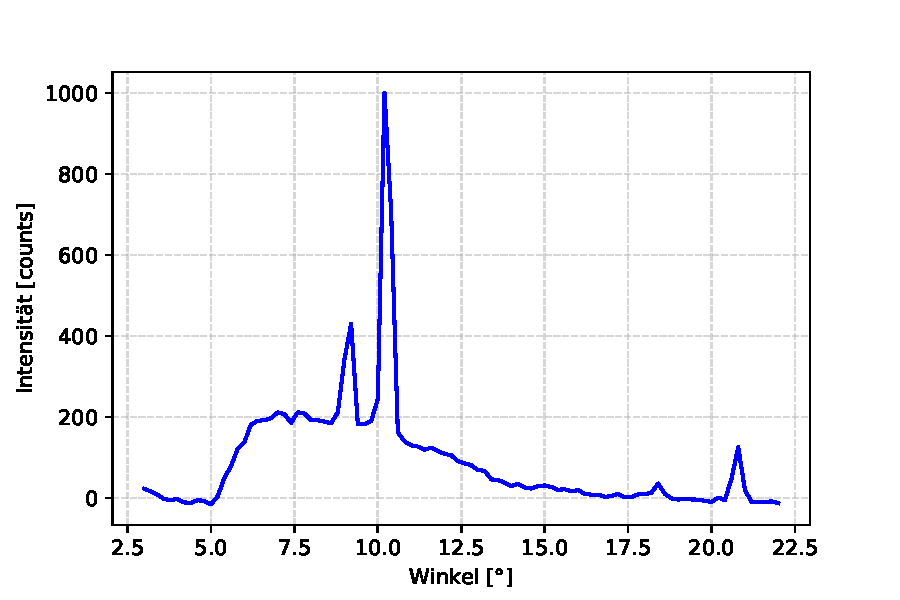
\includegraphics{graphics/plots/A1a.pdf}}
    \caption{Aufgenommenes Röntgenspektrum - LiF-Kristall}
    \label{fig:1a}
\end{figure}

\begin{figure}[!p]
    \centering
    \resizebox{0.9\textwidth}{!}{
    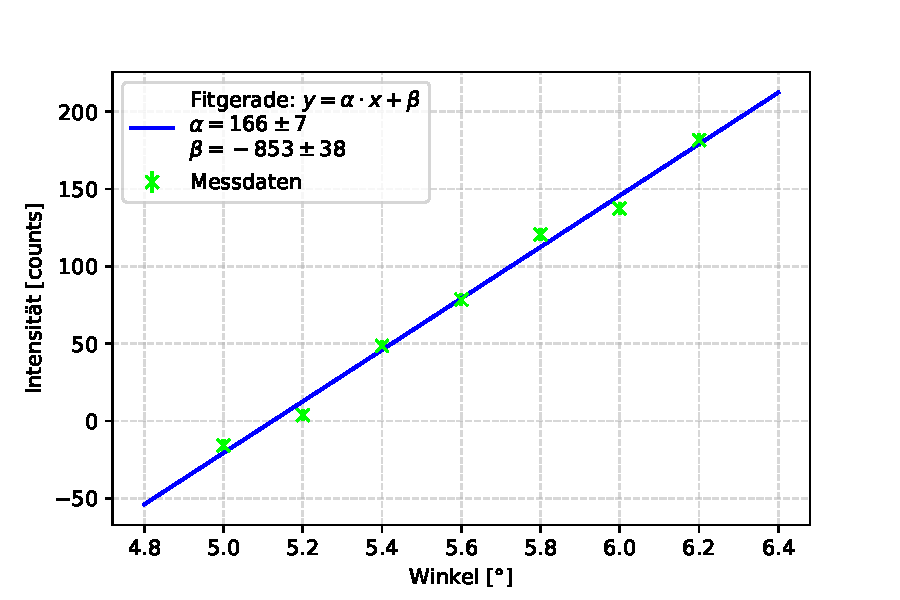
\includegraphics{graphics/plots/A1b.pdf}}
    \caption{Linearer Fit an die Messdaten}
    \label{fig:1b}
\end{figure}

\clearpage
\newpage

\subsection{Analyse der K-Linien 1. und 2. Ordnung}

Wir bestimmen aus unseren Nahaufnahmen der K-Linien zunächst die Peaks der sichtbaren $\alpha$- und $\beta$-Linien, um die Winkel $\theta$ und daraufhin analog zum ersten Teil die Wellenlängen für alle Linien zu erhalten. Die Nahaufnahmen mit eingetragenen Peaks sind in Abbildung \ref{fig:2K-Linien_Peaks} zu sehen. Hierbei ist zu beachten, dass beim Bragg-Gesetz für die Linien zweiter Ordnung der Faktor 1/2 von $n=2$ berücksichtigt wird. Für die Fehler gehen wir folgendermaßen vor: Als Fehler für die ausgelesenen Winkel der Peaks nehmen wir den Abstand zwischen den Messwerten von 0,1° und der Fehler der Wellenlängen berechnet sich wie gewohnt nach Gauß:

\begin{equation}
    \begin{split}
        \Delta \lambda = \frac{2}{n} d \cos{\theta} \cdot \Delta \theta
    \end{split}
\end{equation}

Am Schluss vergleichen wir die Wellenlängen mit dem Literaturwerten von $\lambda_{K_\alpha} = 71,1 \cdot 10^{-12}$ und $\lambda_{K_\beta} = 63,2 \cdot 10^{-12}$. Die Ergebnisse werden alle in Tabelle \ref{tab:K_Linien} eingetragen.

\phantom{.}

\begin{table}[!h]
    \centering
    %\resizebox{\textwidth}{!}{
    \begin{tabular}{ccccc}
        \hline
        \textbf{Ordnung} & \textbf{Linie} & $\bm{\theta}$ [°] & $\bm{\lambda}$ [$10^{-12}$m] & $\bm{\sigma}$  \\ \hline
          1 & $K_\alpha$     & 10,4 $\pm$  0,1 & 72,7 $\pm$ 0,7 & 2,33 \\
          1 & $K_\beta$      & 9,3  $\pm$  0,1 & 65,1  $\pm$ 0,7 & 2,73 \\
          2 & $K_\alpha$     & 20,9 $\pm$  0,1 & 72  $\pm$ 3   & 2,27 \\
          2 & $K_\beta$      & 18,5 $\pm$  0,1 & 64 $\pm$ 3   & 2,12  \\ \hline
    \end{tabular}%}
    \caption{K-Linien des Röntgenspektrums}
    \label{tab:K_Linien}
\end{table}

\phantom{.}

Obwohl die Sigmawerte leicht erhöht sind, liegen alle bestimmten Wellenlängen innerhalb der 3$\sigma$-Umgebung des jeweiligen Literaturwerts und weisen somit keine signifikanten Abweichungen auf. 

Zuletzt fitten wir an die K$_\alpha$-Linie 1. Ordnung eine Gaußfunktion an, um die Halbwertsbreite des Peaks zu bestimmen. Der in Abbildung \ref{fig:2hwb} dargestellte Fit ergibt dabei den Wert:

\begin{equation}
    \sigma = (0,118 \pm 0,007)^\circ.
\end{equation}

Unser zuvor abgeschätzter Fehler von 0,1° anhand des Abstands der Messwerte erscheint also durchaus sinnvoll.

\begin{figure}[!p]
  \centering
  \subfloat[1. Ordnung]{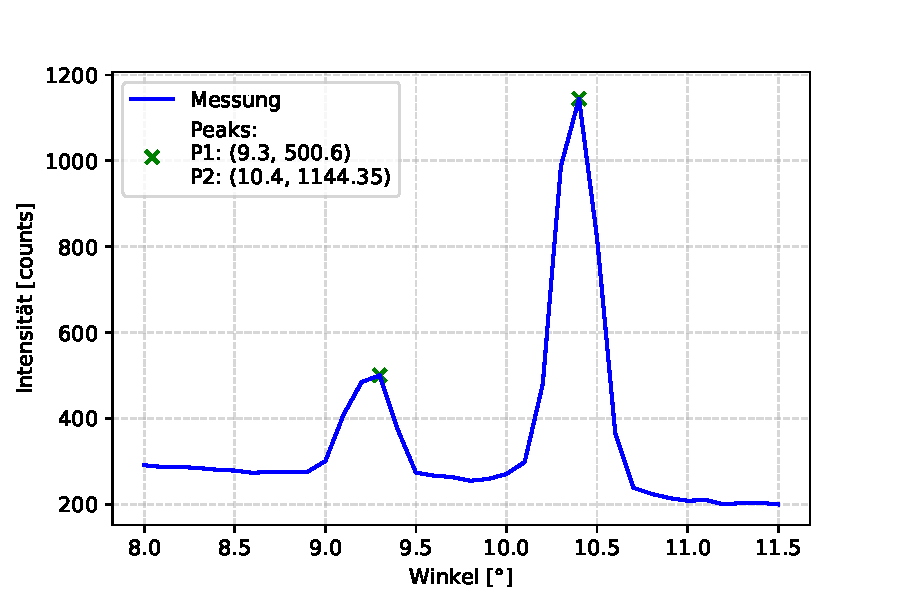
\includegraphics[width=0.9\textwidth]{graphics/plots/A2.1.pdf}}
  \hfill
  \subfloat[2. Ordnung]{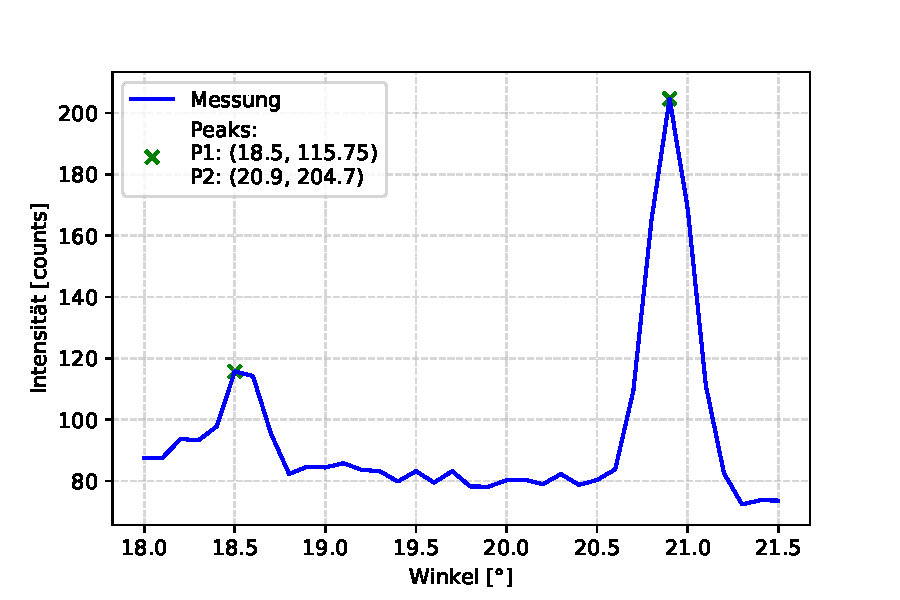
\includegraphics[width=0.9\textwidth]{graphics/plots/A2.2.pdf}}
  \hfill
  \caption{Nahaufnahmen der K-Linien mit eingetragenen Peaks}
  \label{fig:2K-Linien_Peaks}
\end{figure}

\begin{figure}[!p]
    \centering
    \resizebox{0.9\textwidth}{!}{
    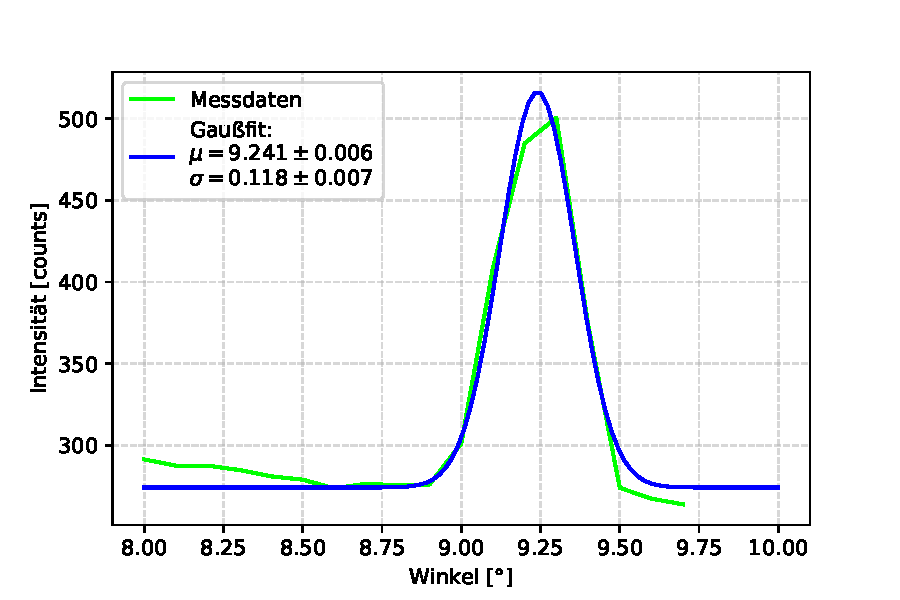
\includegraphics{graphics/plots/A2hwb.pdf}}
    \caption{Gaußfit an die K$_\alpha$-Linie 1. Ordnung}
    \label{fig:2hwb}
\end{figure}

\clearpage
\newpage

\subsection{Analyse der Messung mit verschiedenen Beschleunigungsspannungen}

Zunächst erstellen wir einen Plot mit den in Tabelle 1 des Messprotokoll aufgenommenen Daten der Zählrate gegen die Beschleunigungspannung bei konstantem Beugungswinkel, Abbildung \ref{fig:3_mess}. Wir erkennen den linearen Verlauf ab einer Spannung von ca. 24kV und extrapolieren diesen ähnlich wie im ersten Teil der Auswertung um die Spannung zu bestimmen, ab der Röntgenstrahlung detektiert wird. Der lineare Fit, zu sehen in Abbildung \ref{fig:3_fit}, ergibt die folgenden Parameter:

\begin{equation}
    \begin{split}
        \alpha &= (25,6\pm 0,3) \ \text{1/(kV s)}, \\
        \beta &= -(598 \pm 8) \ \text{1/s}. 
    \end{split}
\end{equation}

Wir berechnen erneut die Nullstele der Funktion und erhalten die Grenzspannung $U_{gr}$:

\begin{equation}
    \begin{split}
        U_{gr} &= - \frac{\beta}{\alpha}, \\
        \Rightarrow \Delta U_{gr} &= -U_{gr} \sqrt{\left( \frac{\Delta \alpha}{\alpha} \right)^2 + \left( \frac{\Delta \beta}{\beta} \right)^2}, \\ \\
        &\Rightarrow U_{gr} = (23,4 \pm 0,4)\text{kV}.
    \end{split}
\end{equation}

Nun können wir mithilfe des eingestellten Winkels von $\vartheta = 7,5$° erneut das Planck'sche Wirkungsquant anhand der Bragg-Gleichung bestimmen:

\begin{equation}
    \begin{split}
        h &= \frac{2de}{c} \ U_{gr} \ \sin \vartheta, \\
        \Rightarrow \Delta h &= \frac{2de}{c} \ \Delta U_{gr} \ \sin \vartheta, \\ \\
        &\Rightarrow \bm{h = (6,57 \pm 0,11) \cdot 10^{-34}} \textbf{Js}.  
    \end{split}
\end{equation}

Wir vergleichen das Ergebnis wieder mit dem Literaturwert und erhalten erneut eine insignifikante Abweichung von $\sigma_h = 0,54$.

\begin{figure}[!p]
    \centering
    \resizebox{0.9\textwidth}{!}{
    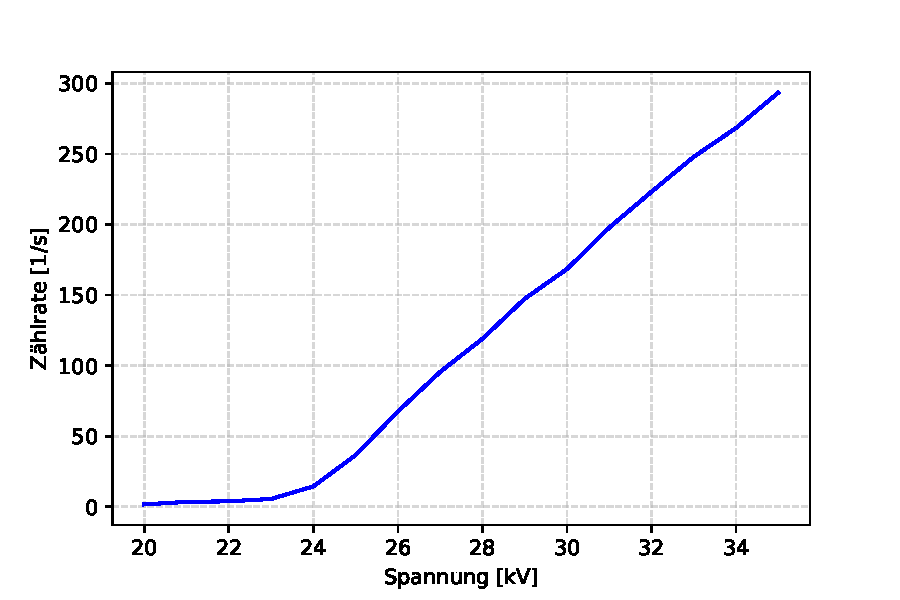
\includegraphics{graphics/plots/A3.1.pdf}}
    \caption{Zählrate als Funktion der Spannung bei festem Winkel}
    \label{fig:3_mess}
\end{figure}

\begin{figure}[!p]
    \centering
    \resizebox{0.9\textwidth}{!}{
    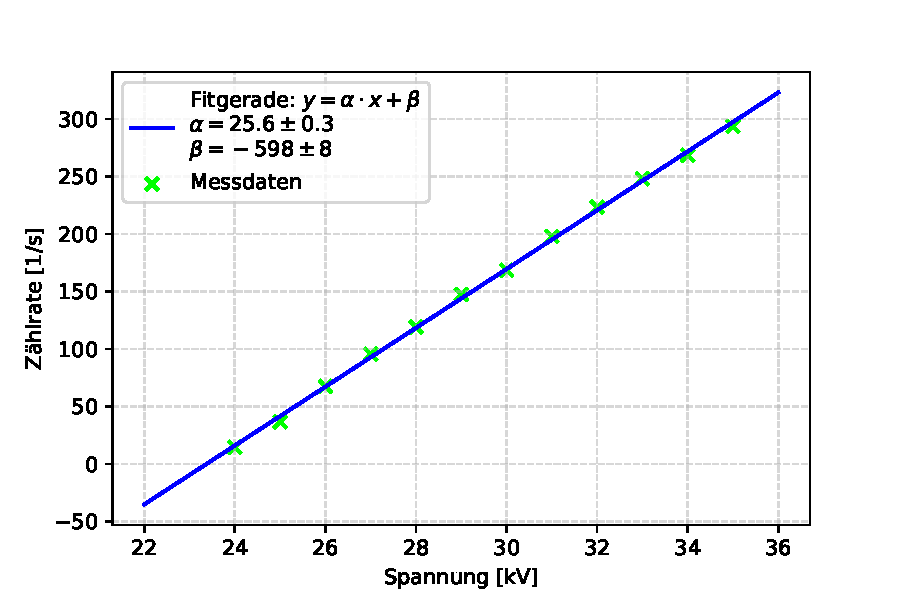
\includegraphics{graphics/plots/A3fit.pdf}}
    \caption{Linearer Fit zur Bestimmung der Grenzspannung}
    \label{fig:3_fit}
\end{figure}

\clearpage
\newpage

\subsection{Auswertung der Messungen mit dem NaCl-Kristall}

Im letzten Teil der Auswertung befassen wir uns mit dem aufgezeichneten Röntgenspektrum unter Verwendung des NaCl-Kristalls im Vergleich zum vorher benutzten LiF-Kristall. Ziel ist die Bestimmung des Netzebenenabstands des Kristalls sowie der Avogadrozahl. Wir beginnen, indem wir aus dem aufgenommenen Spektrum die Peaks der K$_\alpha$- und K$_\beta$-Linien erster und zweiter Ordnung bestimmen. Spektrum und Peaks sind in Abbildung \ref{fig:4_spek} dargestellt. Aus den Winkeln $\theta_{NaCl}$ kann man dann, indem man die Winkel der K-Linien vom LiF-Kristall $\theta_{LiF}$ zur Hilfe nimmt, den Netzebenenabstand berechnen. Dazu teilt man die Bragg-Gleichung für den einen Kristall einfach durch die für den anderen Kristall und erhält, wenn man berücksichtigt, dass $\lambda$ und $n$ für beide gleich sein werden, die folgende Form:

\begin{equation}
    \begin{split}
        \frac{d_{NaCl}}{d_{LiF}} &= \frac{\sin \theta_{LiF}}{\sin \theta_{NaCl}} \ \ \Rightarrow \ \ d_{NaCl} = d_{LiF} \frac{\sin \theta_{LiF}}{\sin \theta_{NaCl}} \\
        \Rightarrow \Delta d_{NaCl} &= d_{NaCl} \left\{ \left( \frac{\cos \theta_{LiF}}{\sin \theta_{NaCl}} \Delta \theta_{LiF} \right)^2 + \ldots \right. \\
        &\left. \phantom{.............} + \left( \frac{\sin \theta_{LiF} \ \cos \theta_{NaCl}}{\sin^2 \theta_{NaCl}} \Delta \theta_{NaCl} \right)^2 \right\}^{1/2}
    \end{split}
\end{equation}

So können wir für alle 4 K-Linien einen Wert für den Netzebenenabstand $d$ bestimmen, was in Tabelle \ref{tab:4K_Netz} verzeichnet ist.

\phantom{.}

\begin{table}[!h]
    \centering
    %\resizebox{\textwidth}{!}{
    \begin{tabular}{ccccc}
        \hline
        \textbf{Ordnung} & \textbf{Linie} & $\bm{\theta_{NaCl}}$ [°] & $\bm{\theta_{LiF}}$ [°]  & $\bm{d_{NaCl}}$ [pm] \\ \hline
              1 & $K_\alpha$    &     7.2 $\pm$ 0.1 &   10.4 $\pm$ 0.1 & 290 $\pm$ 5 \\
              1 & $K_\beta$     &     6.2 $\pm$ 0.1 &    9.3 $\pm$ 0.1 & 288,9 $\pm$ 2.4 \\
              2 & $K_\alpha$    &    14.4 $\pm$ 0.1 &   20.9 $\pm$ 0.1 & 301 $\pm$ 6 \\
              2 & $K_\beta$     &    12.8 $\pm$ 0.1 &   18.5 $\pm$ 0.1 & 288,4 $\pm$ 2.7 \\ \hline
    \end{tabular}%}
    \caption{NaCl - K-Linien und Netzebenenabstand}
    \label{tab:4K_Netz}
\end{table}

\phantom{.}

Wir berechnen den Mittelwert $\overline{d}_{NaCl}$ aus den berechneten Netzebenenabständen, wobei sich der Mittelwert aus dem Standardfehler sowie den Fehlern der einzelnen Werte folgendermaßen ergibt:

\begin{equation}
    \begin{split}
        \Delta \overline{d}_{NaCl} &= \sqrt{\sigma_{std}^2 + \left( \frac{1}{N} \sum_{i=1}^N \Delta d_i \right)^2} \\
        \text{mit} \ \ \ \sigma_{std} &= \sqrt{\frac{1}{N(N-1)} \sum_{i=1}^N (\overline{d} - d_i)^2}.
    \end{split}
\end{equation}

Somit kommen wir auf das folgende Ergebnis für den Netzebenenabstand vom NaCl-Kristall:

\begin{equation}
    \bm{\overline{d}_{NaCl} = (292 \pm 5)} \textbf{pm}.
\end{equation}

Damit können wir nun gemäß Gleichung \ref{eq:1_AVOGADRO} die Avogadrozahl $NA$ bestimmen. Wir verwenden die im Skript gegebenen Werte der Molmasse $M = 58,44$g und Dichte $\rho = 2,164$g/cm$^3$ von NaCl und erhalten:

\begin{equation}
    \begin{split}
        NA &= \frac{1}{2} \frac{M}{\rho \ \overline{d}_{NaCl}^3}, \\
        \Rightarrow \Delta NA &= NA \sqrt{\left( 3 \frac{\Delta \overline{d}_{NaCl}}{\overline{d}_{NaCl}} \right)^2}, \\ \\
        &\Rightarrow \bm{NA = (5,41 \pm 0,28) \cdot 10^{23}} \ \textbf{1/mol}.
    \end{split}
\end{equation}

Verglichen mit dem Literaturwert von $NA_{lit} = 6,0221 \cdot 10^{23}$ 1/mol ergibt sich eine zwar leicht erhöhte aber immer noch insignifikante Abweichung von $\sigma_{NA} = 2,20$.

\begin{figure}[!p]
    \centering
    \resizebox{0.9\textwidth}{!}{
    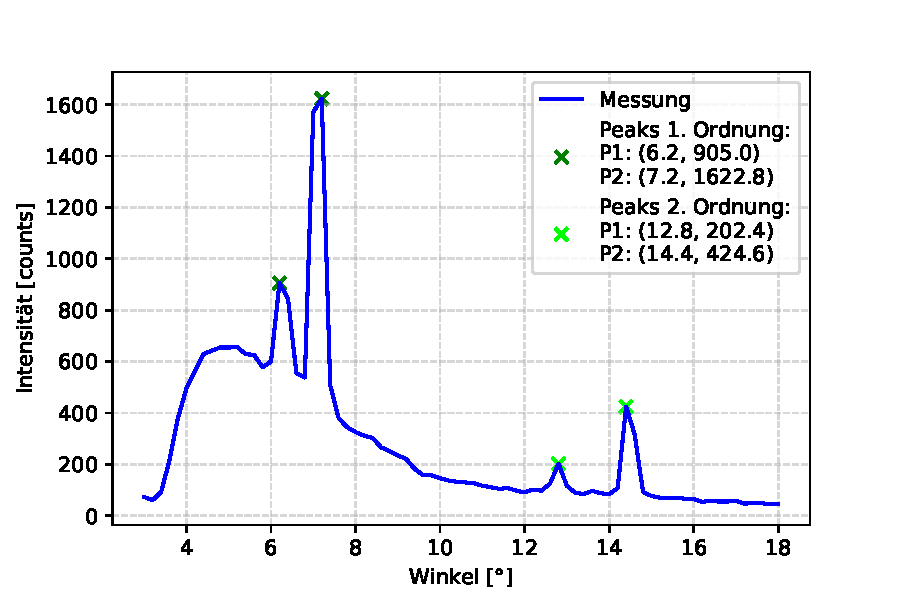
\includegraphics{graphics/plots/A4.pdf}}
    \caption{Röntgenspektrum des NaCl-Kristalls mit Peaks}
    \label{fig:4_spek}
\end{figure}

\clearpage
\newpage
%---------------PRÄSENTATION DER ENDERGEBNISSE---------------
\section{Zusammenfassung der Endergebnisse}

Wir begannen, indem wir aus der Aufnahme des gesamten Röntgenspektrums des LiF-Kristalls das Planck'sche Wirkungsquant sowie den Startwinkel des charakteristischen Spektrums zweiter Ordnung bestimmten. Wir erhielten dabei:

\begin{equation}
    \begin{split}
        h &= (6,7 \pm 0,4) \cdot 10^{-34} \text{Js} \\
        \vartheta_{gr,2} &= (10,3 \pm 0,6)^\circ
    \end{split}
\end{equation}

Der Wert für $h$ lag mit einer Sigmaabweichung von 0,25 nah am Literaturwert, was ein einwandfreies Ergebnis mit einer akzeptablem Fehlergröße darstellt. Der Startwinkel zeigt im Kontext der Aufnahme die Überlappung der Ordnungen, da bei dem berechneten Wert noch Linien erster Ordnung vorzufinden sind.

Daraufhin bestimmten wir die Wellenlängen der K-Linine erster und zweiter Ordnung und verglichen auch diese mit den Literaturwerten. Auch hier lagen alle Werte innerhalb insignifikanter Abweichungen von den gegeben Literaturwerten. 

Anschließend berechneten wir aus unserer Spannungsmessung bei festem Winkel erneut das Planck'sche Wirkungsquant und erzielten das folgende Ergebnis:

\begin{equation}
    h = (6,57 \pm 0,11) \cdot 10^{-34} \text{Js}
\end{equation}

Mit einer Sigmaabweichung von 0,54 weist auch dieser Wert keine signifikante Abweichung vom Literaturwert auf. 

Zuletzt werteten wir unsere Aufnahme des NaCl-Kristalls aus um den Netzebenenabstand und die Avogadrozahl zu bestimmen. Wir bekamen:

\begin{equation}
    \begin{split}
        \overline{d}_{NaCl} &= (292 \pm 5) \text{pm} \\
        NA &= (5,41 \pm 0,28) \cdot 10^{23} \ \text{1/mol}
    \end{split}
\end{equation}

Für den Wert der Avogradozahl ergab der Signifiknaztest eine Abweichung von 2,20. Somit ist auch hier keine signifikante Abweichung vorhanden. 



\newpage
%---------------ZUSAMMENFASSUNG UND DISKUSSION---------------
\section{Diskussion}

Die Endergebnisse sind im allgemeinen durchaus zufriedenstellend und passen gut zu der grundlegenden Theorie. Der Fakt, dass keine signifikante Abweichung oberhalb der 3$\sigma$-Umgebung vorliegt ist eine aussagekräftige Bestätigung der verwendeten Methoden und physikalischen Gesetze. 

Im ersten Teil bestätigen sich die in der Einleitung hergeleiteten Konzepte der Grenzwellenlänge sowie des Bragg-Gesetzes und zeigt, dass dies ein einfacher und effektiver Weg ist, das Planck'sche Wirkungsquant zu bestimmen. Bezüglich des berechneten Startwinkels haben wir zwar keine quantitative Bewertung, da einfach ein Vergleichswert fehlt, jedoch kann man sagen, dass die positiven Ergebnisse der anderen Werte diese bestätigen und somit der Startwinkel, der sich aus diesen bestätigten Ergebnissen zusammensetzt, nicht allzu verkehrt sein sollte. Somit lassen sich im Endeffekt als potentielle Fehlerquellen nur allgemeinere Messungenauigkeiten nennen, welche für die standardmäßigen Abweichungen gesorgt haben. 

Im zweiten Teil lässt sich feststellen, dass alle bestimmten Wellenlängen ein wenig größer sind als die jeweiligen Literaturwerte, was wohl der Grund für die leicht erhöhten (aber immer noch insignifikanten) Sigmaabweichungen sein wird. Dies lässt auf einen kleineren systematischen Fehler schließen, welcher am Wahrscheinlichsten entweder von der Messung oder sogar dem Messgerät selbst stammen wird. Da sich die Abweichungen aber wie gesehen in Grenzen halten belassen wir es hier bei der kurzen Erwähnung der Beobachtung.

Im dritten Teil fällt auf, das unser berechneter Wert des Planck'schen Wirkungsquants mehr vom Literaturwert abweicht als im ersten Teil. Dies ist zunächst unerwartet, da die hier verwendete Isochromatenmethode eigentlich genauer sein sollte als die vorherige Extrapolation. Potentielle Fehlerquellen könnten hier Ungenauigkeiten in Messdaten der Zählraten oder andere statistische Schwankungen sein. Im Allgemeinen ist das Ergebnis aber wie gesagt sehrt akzeptabel, einzig und allein der Vergleich zum ersten Teil wirkte auffällig, ist aber auch nicht weiter von Belangen.

Im letzten Teil zeigt sich im Endergebnis eine leicht erhöhte Abweichung. Auffällig ist der Netzebenenabstand, der aus der K$_\alpha$-Linie zweiter Ordnung bestimmt wurde, da dieser deutlich oberhalb der anderen liegt. Woher genau diese starke Abweichung der einen Linie kommt lässt sich nur schwer sagen, da es aber nur diese eine Linie betrifft wäre ein zufälliger statistischer Fehler denkbar. Der erhöhte Wert sorgt für einen größeren Mittelwert des Netzebenenabstands und damit für einen zu kleinen Wert der Avogadrozahl, was genau der Fall beim Endergebnis ist. Somit kamen wir auf das leicht zu kleine Ergebnis, welches aber immer noch innerhalb der $3\sigma$-Umgebung vom Literaturwert liegt.

Abschließend lässt sich also sagen, dass durchweg zufriedenstellende Ergebnisse erzielt wurden, welche die Theorie bestätigen und das Experiment zu einem einfach und interessanten Weg machen, grundlegende Physikalische Konstanten zu Bestimmen und eine Einführung in die Grundlagen der Röntgenspektroskopie zu geben. 



\newpage
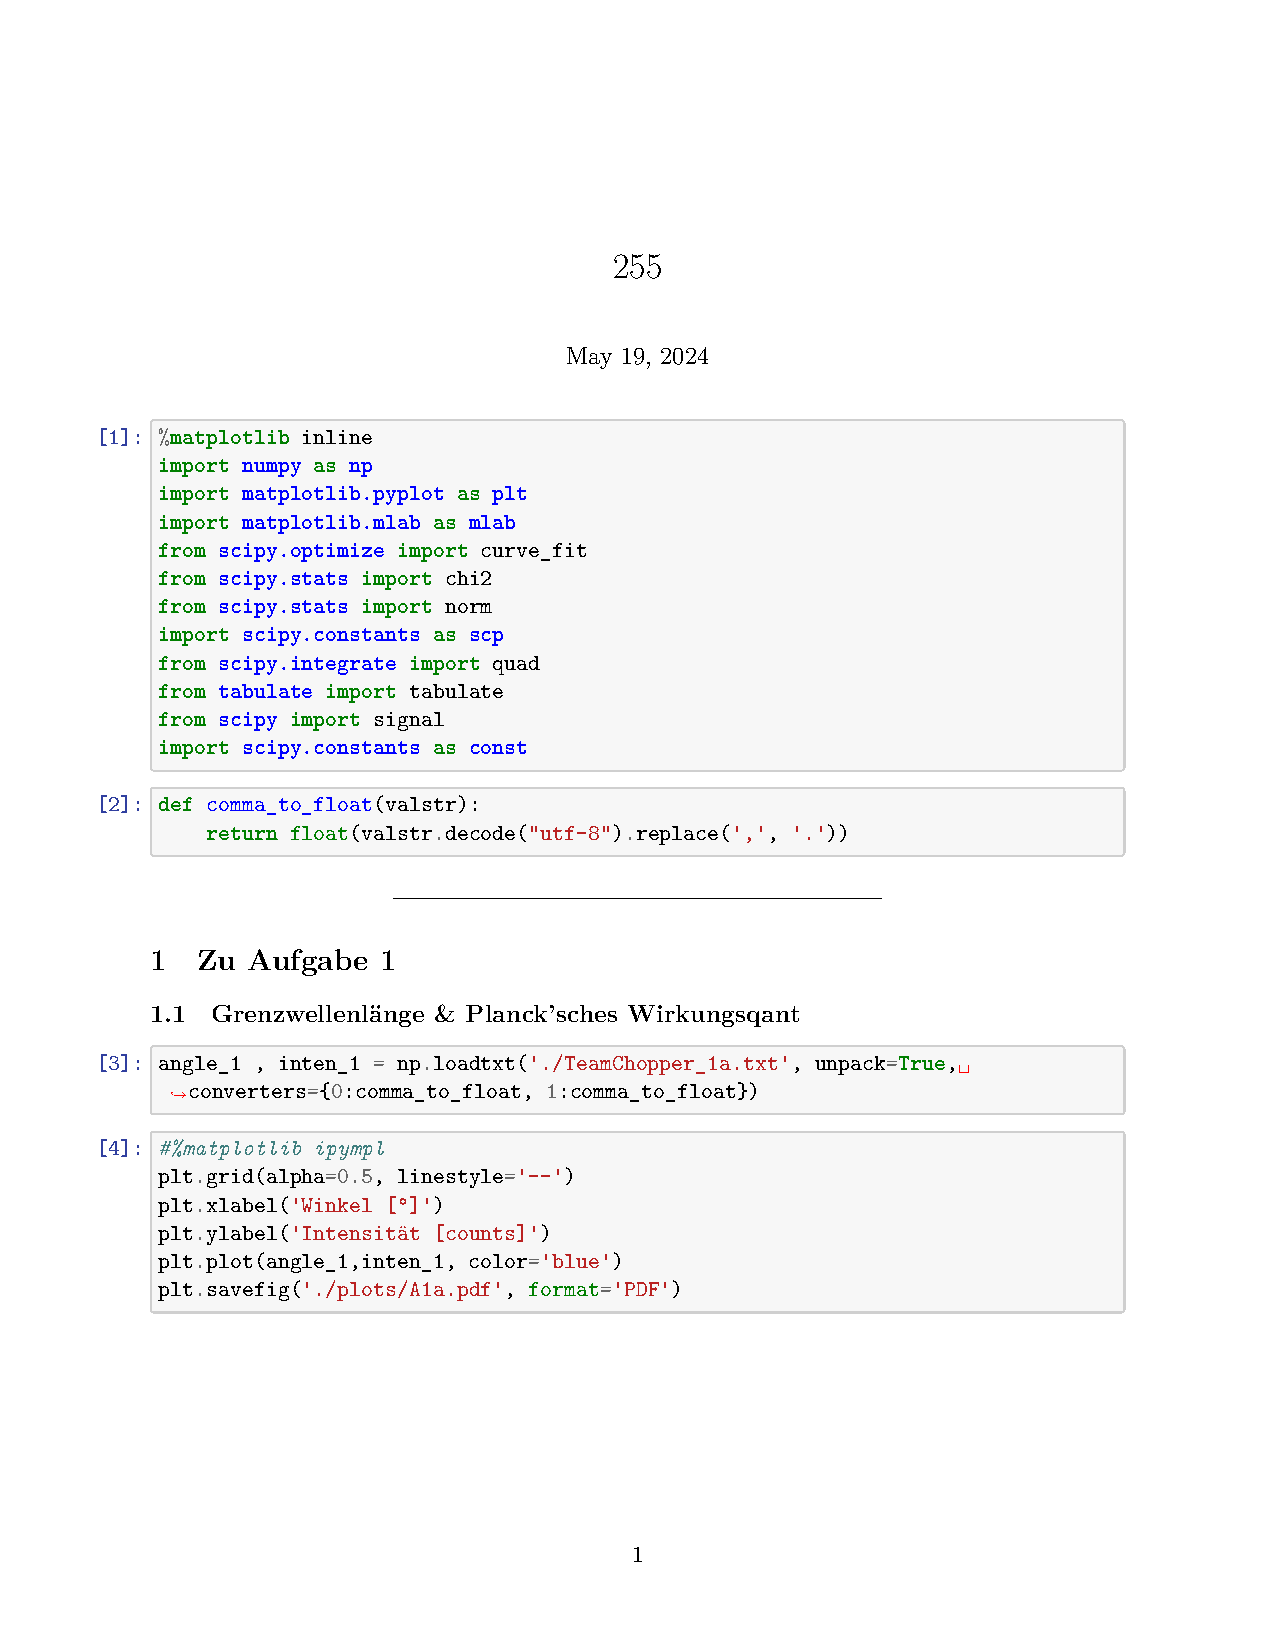
\includepdf[pages=-]{255.pdf}

\end{document}

